\documentclass[fleqn]{beamer}
\usepackage{amsmath}
\mode<presentation> {
\usepackage{threeparttable}
\RequirePackage{siunitx}
\usepackage{tabulary}
\usepackage{float}
\usepackage{graphicx}
\usepackage{subfig}
\newcommand{\wmi}{\ensuremath{W_{b_m}\left(\frac{x-Y_{t_i}}{b_m}\right) }\xspace}
\newcommand{\wmj}{\ensuremath{W_{b_m}(({x-Y_{t_i}})/{b_m}) }\xspace}
\newcommand{\kmj}{\ensuremath{K(({x-X_{t_i}})/{b_m}) }\xspace}
\newcommand{\kmi}{\ensuremath{K\left(\frac{X_{t_i} - x}{b_m}\right) }\xspace}
\newcommand{\Xtm}{\ensuremath{X_{t-}}\xspace}
\newcommand{\sbm}{\ensuremath{W}\xspace}
\newcommand{\etn}{\ensuremath{\varepsilon_i^{T_n}}\xspace}
\newcommand{\Wbn}{\ensuremath{W_{b_n}}\xspace}
\newcommand{\ms}{\ensuremath{m^*}\xspace}
\newcommand{\Rs}{\ensuremath{R^*}\xspace}
\newcommand{\lw}{\ensuremath{{L}^W_n(x, T)}\xspace}
\newcommand{\lk}{\ensuremath{{L}^K_n(x, T)}\xspace}
\newcommand{\iid}{i.i.d\xspace}
\newcommand{\ito}{It\^o\xspace}
\newcommand{\lbm}{\ensuremath{(\triangle_m\ln(1/\triangle_m))}\xspace}
\newcommand{\lbn}{\ensuremath{(\triangle_n\ln(1/\triangle_n))}\xspace}
\renewcommand{\i}{\mathrm{i}} 
\newcommand{\sumn}{\ensuremath{\sum_{k \in \nats}}\xspace}
\newcommand{\sumin}{\ensuremath{\sum_{i = 0}^{n-1}}\xspace}
\newcommand{\sumi}{\ensuremath{\sum_{k \in \ints}}\xspace}
\newcommand{\sumt}{\ensuremath{\sum_{(h,k) \in \Theta_n}}\xspace}
\newcommand{\sv}{\ensuremath{\sigma^2}\xspace}
\newcommand{\bsv}{\ensuremath{\bar{\sigma}^2}\xspace}
\newcommand{\svnt}{\ensuremath{\sigma^2}\xspace}
\newcommand{\svhk}{\ensuremath{\sigma^2_{h,k}}\xspace}
\newcommand{\vh}{\ensuremath{V_h(\phi)}\xspace}
\newcommand{\idp}{\ensuremath{\mu}\xspace}
\newcommand{\svn}{\ensuremath{\hat{\sigma}_{n}^2}\xspace}
\newcommand{\Svn}{\ensuremath{\hat{\Sigma}_n}\xspace}
\newcommand{\svnb}{\ensuremath{\hat{\sigma}_{n,b}^2}\xspace}
\newcommand{\svnN}{\ensuremath{\hat{\sigma}_{t}^2}\xspace}
\newcommand{\hs}{\ensuremath{\mcal{H}}\xspace}
\newcommand{\T}{\ensuremath{\tau}\xspace}
\newcommand{\chk}{\ensuremath{{c}_{h,k}}\xspace}
\newcommand{\cnhk}{\ensuremath{\hat{c}_{h,k}}\xspace}
\newcommand{\ivp}{\ensuremath{\sigma}\xspace}
\newcommand{\inner}[2]{\ensuremath{\langle{#1},{#2}\rangle}\xspace}
\newcommand{\hn}[1]{\ensuremath{\vert{#1}\vert_{\calpha}}\xspace}
\newcommand{\ghk}{\ensuremath{g_{h,k}}\xspace}
\newcommand{\tghk}{\ensuremath{\tilde{g}_{h,k}}\xspace}
\newcommand{\btghki}{\ensuremath{\overline{\tilde{g}_{h,k}(t_i)}}\xspace}
\newcommand{\btghks}{\ensuremath{\overline{\tilde{g}_{h,k}(s)}}\xspace}
\newcommand{\tg}{\ensuremath{\tilde{g}}\xspace}
\newcommand{\czero}{\ensuremath{C^0[0,1]}\xspace}
\newcommand{\domain}{\ensuremath{[0,1]}\xspace}
\newcommand{\calpha}{\ensuremath{C^{0,\alpha}[0,1]}\xspace}
\newcommand{\state}{\czero}
\newcommand{\hkints}{\ensuremath{h,k \in \ints}\xspace}
\newcommand{\mise}{integrated mean aquare error\xspace}
\newcommand{\isqb}{integrated square bias\xspace}

% The Beamer class comes with a number of default slide themes
% which change the colors and layouts of slides. Below this is a list
% of all the themes, uncomment each in turn to see what they look like.

%\usetheme{default}
%\usetheme{AnnArbor}
%\usetheme{Antibes}
%\usetheme{Bergen}
%\usetheme{Berkeley}
%\usetheme{Berlin}
%\usetheme{Boadilla}
%\usetheme{CambridgeUS}
%\usetheme{Copenhagen}
%\usetheme{Darmstadt}
%\usetheme{Dresden}
%\usetheme{Frankfurt}
%\usetheme{Goettingen}
%\usetheme{Hannover}
%\usetheme{Ilmenau}
%\usetheme{JuanLesPins}
%\usetheme{Luebeck}
%\usetheme{Madrid}
%\usetheme{Malmoe}
%\usetheme{Marburg}
%\usetheme{Montpellier}
%\usetheme{PaloAlto}
%\usetheme{Pittsburgh}
%\usetheme{Rochester}
%\usetheme{Singapore}
%\usetheme{Szeged}
%\usetheme{Warsaw}

% As well as themes, the Beamer class has a number of color themes
% for any slide theme. Uncomment each of these in turn to see how it
% changes the colors of your current slide theme.

%\usecolortheme{albatross}
%\usecolortheme{beaver}
%\usecolortheme{beetle}
%\usecolortheme{crane}
%\usecolortheme{dolphin}
%\usecolortheme{dove}
%\usecolortheme{fly}
%\usecolortheme{lily}
%\usecolortheme{orchid}
%\usecolortheme{rose}
%\usecolortheme{seagull}
%\usecolortheme{seahorse}
%\usecolortheme{whale}
%\usecolortheme{wolverine}

%\setbeamertemplate{footline} % To remove the footer line in all slides uncomment this line
%\setbeamertemplate{footline}[page number] % To replace the footer line in all slides with a simple slide count uncomment this line

%\setbeamertemplate{navigation symbols}{} % To remove the navigation symbols from the bottom of all slides uncomment this line
}
\usepackage{graphicx} % Allows including images
\usepackage{booktabs} % Allows the use of \toprule, \midrule and \bottomrule in tables
%----------------------------------------------------------------------------------------
%	TITLE PAGE
%----------------------------------------------------------------------------------------

\title[Short title]{Estimating realized spot  volatility with Gabor frames.} % The short title appears at the bottom of every slide, the full title is only on the title page
\author{Wale Dare} % Your name
\institute[University of St. Gallen] % Your institution as it will appear on the bottom of every slide, may be shorthand to save space
{
University of St. Gallen \\ % Your institution for the title page
\medskip
%\textit{wale.dare@student.unisg.ch} % Your email address
}
\date{\today} % Date, can be changed to a custom date
\begin{document}
\begin{frame}
\titlepage % Print the title page as the first slide
\end{frame}
\begin{frame}
  \frametitle{Motivation: (Co)volatility ($\sigma^2$) is important}
\begin{enumerate}
  \item Risk management: VaR, CVaR, etc\ldots
  \item Portfolio optimization: Mean-variance optimization 
  \item Option pricing: Black-Scholes formula
  \item etc\ldots
\end{enumerate}
\tableofcontents % Throughout your presentation, if you choose to use \section{} and \subsection{} commands, these will automatically be printed on this slide as an overview of your presentation
\end{frame}
%----------------------------------------------------------------------------------------
%	PRESENTATION SLIDES
%----------------------------------------------------------------------------------------

%------------------------------------------------
%------------------------------------------------
\begin{frame}
  \frametitle{Motivation: Semimartingales as prices}
  \begin{enumerate}
\item 
  Only a security market with prices that evolve as semimartingales can be priced. Delbean \& Schachermayer (1998)
\item  $X$ is a semimartingale on $(\Omega, \mathcal{F}, \mathcal{F}_t, P)$ if there is a finite variation process $A$ and a local martingale $M$ s.t. 
\begin{align} 
    X_t & = A_t + M_t \notag\\
    \only<2->{& = A^c_t+ A^J_t + M^c_t + M^J_t }
    \label{}
  \end{align}
  \end{enumerate}
\end{frame}
\begin{frame}
\frametitle{Ito Semimartingales}
If $X$ has no fixed (Markov) jump times, then 
\begin{align}
  \only<2->{X_t & =  \int^t_0 b_s d s + A^J_t + \int^t_0 \sigma_s d W_s  + M^J_t \notag}
\only<3->{\\& =  \int^t_0 b_s d s +  \int^t_0 \int_{\{\vert x \vert > 1\}} x \mu(dt, dx) \notag \\ & \quad + \int^t_0 \sigma_s d W_s + \int^t_0 \int_{\{\vert x \vert \le  1\}}x[\mu(dt, dx) - dt \nu(dx)] \notag}
  \label{}
\end{align}
\only<4->{$\sigma$, $b$ are stochastic processes. $\mu$ is a measure-valued random variable, i.e. $\mu: \Omega\times \mathcal{B}(\mathbb{R}_+ \times \mathbb{R}) \to \mathbb{R}$, and $\nu$ is its Levy intensity measure.}
\end{frame} 
\begin{frame}
\frametitle{The problem}
%\subsection{What is the efficient price}
\begin{enumerate}
  \item Discrete observations $X_1, \cdots, X_n$ from 
    \begin{align}
      X_t = \int_0^t b_s d s + \int_0^t \sigma_s d W_s + A_t^J + M^J_t, \qquad \forall t \ge 0\notag
      \label{}
    \end{align} over a fixed interval $[0,T]$
  \item Estimate $\sigma^2$ over the interval $[0,T]$.
    \begin{enumerate}
      \item Nonparametrically: Arbitrary functional specification
      \item Globally: find a sequence of random \emph{functions} $\hat{\sigma}_n^2:\Omega\times [0,T] \to \mathbb{R}$ s.t.  $\Vert \hat{\sigma}_n^2 - \sigma^2\Vert_{L^2} \to 0$  in probability. (possibly in $L^p$, $p > 1$). 
    \end{enumerate}
\end{enumerate}
\end{frame}
\begin{frame}[allowframebreaks]
  \frametitle{General approach}
  \begin{enumerate}
    \item Assume $\sigma^2 \in L^2[0, T]$, a.s., where 
      \begin{align}
        L^2[0,T] = \left\{ f \in \mathbb{C}^{[0,T]}: \int^T_0 f(s) \bar{f(s)} d s < \infty\right\}
      \end{align}
      is a Hilbert space, so it behaves just like $\mathbb{R}^2$. In particular, the idea of an orhogonal basis ( just like $\{(1,0), (0,1)\}$ in $\mathbb{R}^2$) makes sense in $L^2$.  
    \item If $\{\psi_k\}_{k =1}^\infty$ is such an orthogonal basis and  $f \in L^2$, then there is a sequence of constants $c := \{c_k\}_{k = 1}^\infty$ s.t. $f = \sum_k^{\infty} c_k \psi_k$. 
    In particular,  
      \begin{align}
        \sigma^2(t)  &= \sum_k^{\infty} c_k \psi_k(t) \qquad t \in [0,T]\notag\\
        \label{}
      \end{align}
      where 
      \begin{align}
        c_k = \langle \sigma^2 , \psi_k\rangle : = \int^T_0 \sigma^2(s) \bar{\psi}_k(s) d s\notag
        \label{}
      \end{align}
    \item Examples of $\{\psi_k\}_{k =1}^\infty$: B-Splines, Fourier series (basis), wavelets, etc\dots 
    \item Given discrete $X_i$ at times $t_i$ for $i = 0, \dots, n-1$.
      \begin{align}
        &\hat{\sigma}^2_n  = \sum_h^H \hat{c}_h \psi_h\notag\\
        &\hat{c}_h = \sum^n_{i = 0} \bar{\psi}_h(t_i)(X_{i +1} - X_i)^2 
        \label{}
      \end{align}
  \end{enumerate}
\end{frame}
\begin{frame}
  \frametitle{Previous solutions}
   \begin{enumerate}
    \item Fourier orthogonal basis (Malliavin et. al 2007)
    \item Wavelet orthogonal basis (Hoffmann et al 2012)
  \end{enumerate}
  Consistent ONLY if $X_t$ is a continuous Ito Semimartingale.
  That is \begin{align}
    X_t = \int^t_0 b_s d s + \int^t_0 \sigma_s d W_s. \notag
    \label{}
  \end{align}
\end{frame}
\begin{frame}
  \frametitle{Our contribution}
  \begin{enumerate}
    \item Consistent estimate for the general case in which you have jumps in addition to the continuous part. 
    \begin{align}
        X_t = \int^t_0 b_s d s + \int^t_0 \sigma_s d W_s + A_t^J + M_t^J. \notag
    \label{}
  \end{align}
    \item Generalization of the previous methods based on orthonomal basis. We use frames which generalize the concept of orthogonal basis.
    \item The extension to frames is not just a technical extension, frames, Gabor frames in particular, possess coefficient noise reduction capabilities not found in orthonormal basis.  
  \end{enumerate}
\end{frame}
\begin{frame}
  \frametitle{Frames}
  \begin{enumerate}
    \item They come in pairs: $\{\psi_k\}$ and $\{\tilde{\psi}_k\}$.
    \item Together, they possess the representation property: If $f \in L^2$ then
      \begin{align}
        f = \sum_k c_k  \psi_k \notag
        \label{}
      \end{align}
      where
      \begin{align}
        c_k = \langle f, \tilde{\psi}_k\rangle \notag
        \label{}
      \end{align}
    \item An orthonormal basis is a frame such that $\psi_k = \tilde{\psi}_k$.
  \end{enumerate}

\end{frame}
\begin{frame}
  \frametitle{Gabor frames}
  \begin{enumerate}
    \item They are frames constructed by translating a single function $g$ in time and frequency:
      \begin{align}
        \{g_{h,k}(t) \} :=  \{e^{2\pi i h a t}g(t -k b)\}, \qquad h, k \in \mathbb{Z} \notag
        \label{}
      \end{align}
    \item If $g$ satisfies the partition of unity property then its dual  $\tilde{g}$ is a finite linear combination of translates of $g$, so it is easy to compute.
  \end{enumerate}   
\end{frame}
\begin{frame}
  \frametitle{Nonparametric jump-robust global spot volatility estimator}
\begin{align}
  &\hat{\sigma}^2_n  = \sum_{\vert h \vert < H_n, \vert k\vert < K_0 } \hat{c}_{h,k} g_{h,k}\notag\\
  &\hat{c}_{h,k} = \sum^n_{i = 0} \bar{\tilde{g}}_{h,k}(t_i)(X_{i +1} - X_i)^2I_{\{\vert X_{i + 1} - X_i\vert < u_n\}} 
        \label{}
      \end{align}
      where 
      \begin{enumerate}
        \item 
          $K_0$ is a constant
        \item
      $H_n = O(\sqrt{T/n})$
    \item
      $\frac{\sqrt{(T/n) \log(n/T)}}{u_n} = o(1)$.
      \end{enumerate}
      
\end{frame}
\begin{frame}[allowframebreaks]
  \frametitle{Performance}
  \normalsize{
    \begin{figure}
  \caption{Estimated vs. actual spot volatility}
  \centering
  %\subfloat[ABM]{{ 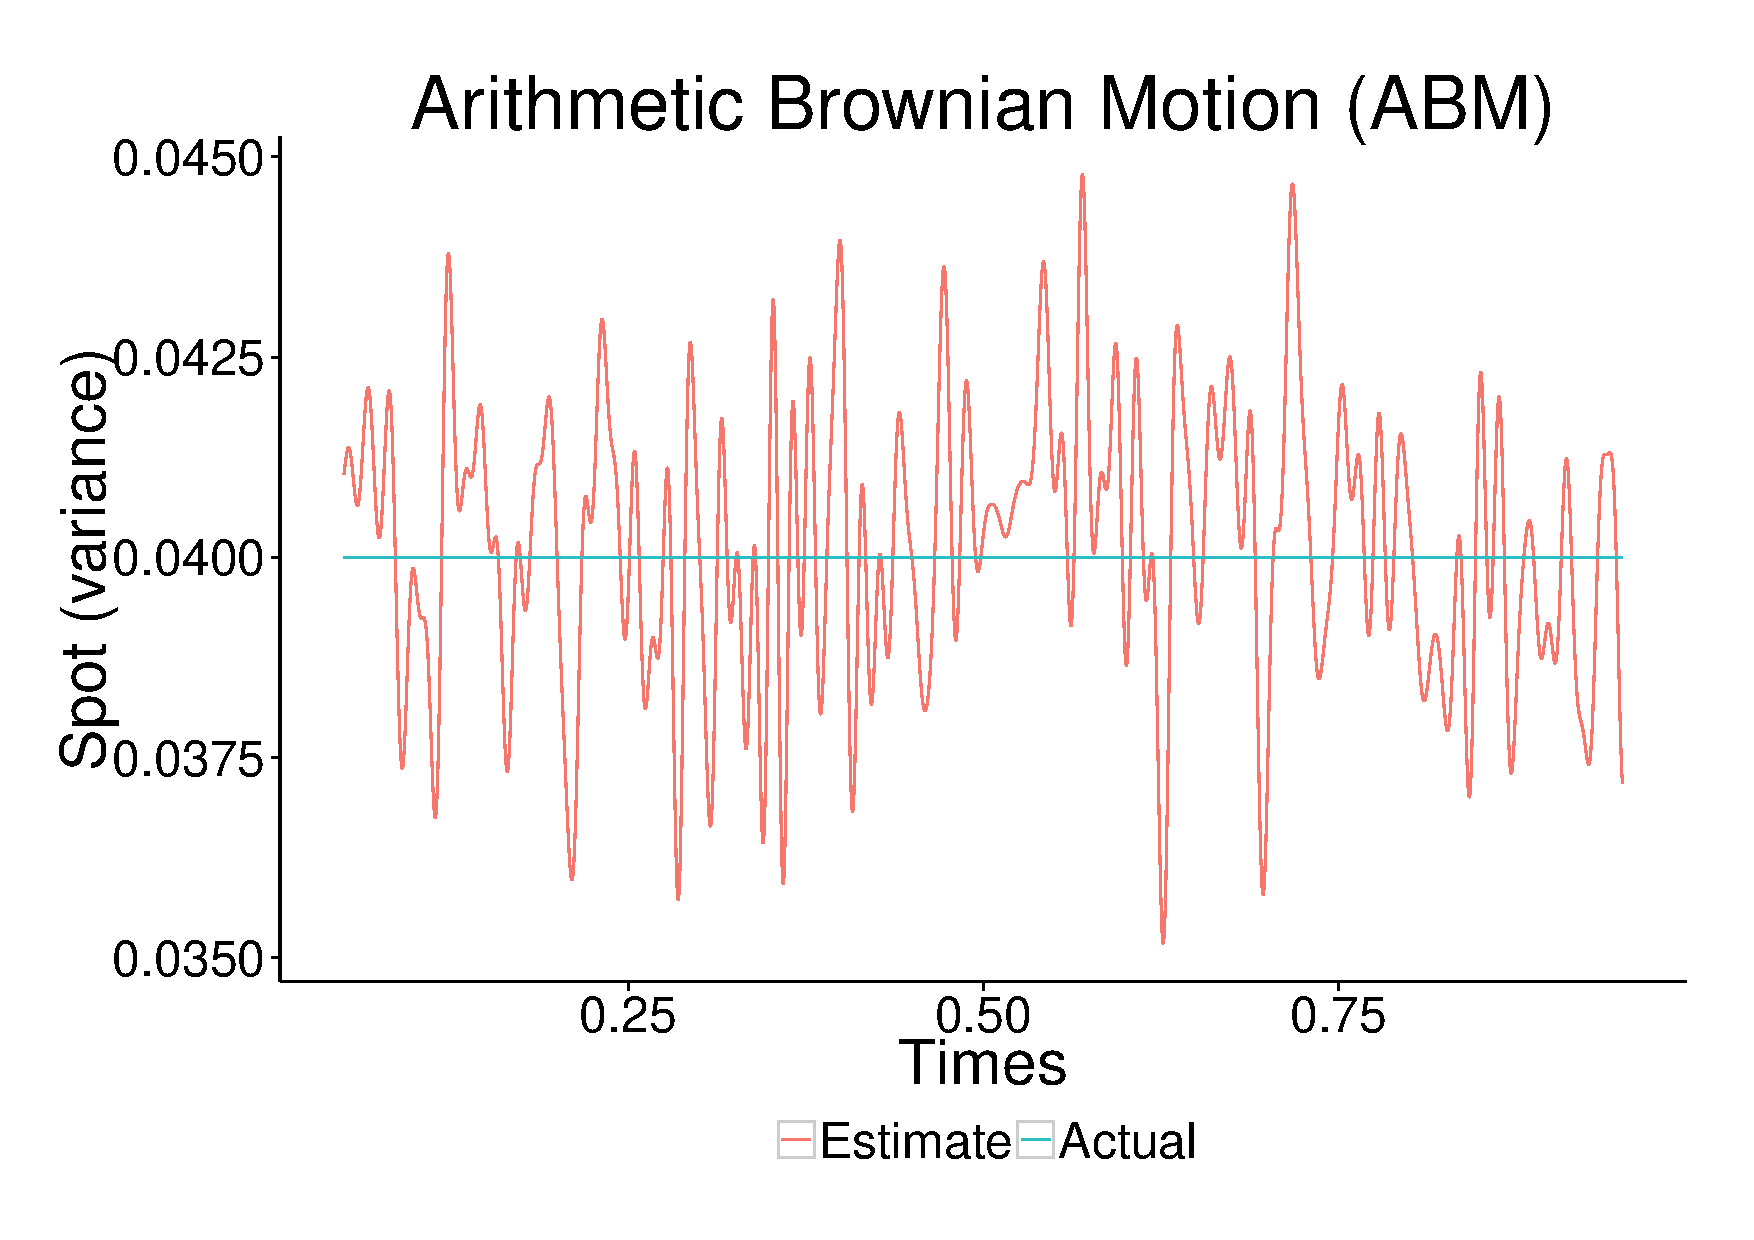
\includegraphics[angle=270,width=0.45\textwidth,totalheight=0.30\textheight]{Simulation/pa.pdf}}}
  \subfloat[GBM]{{ 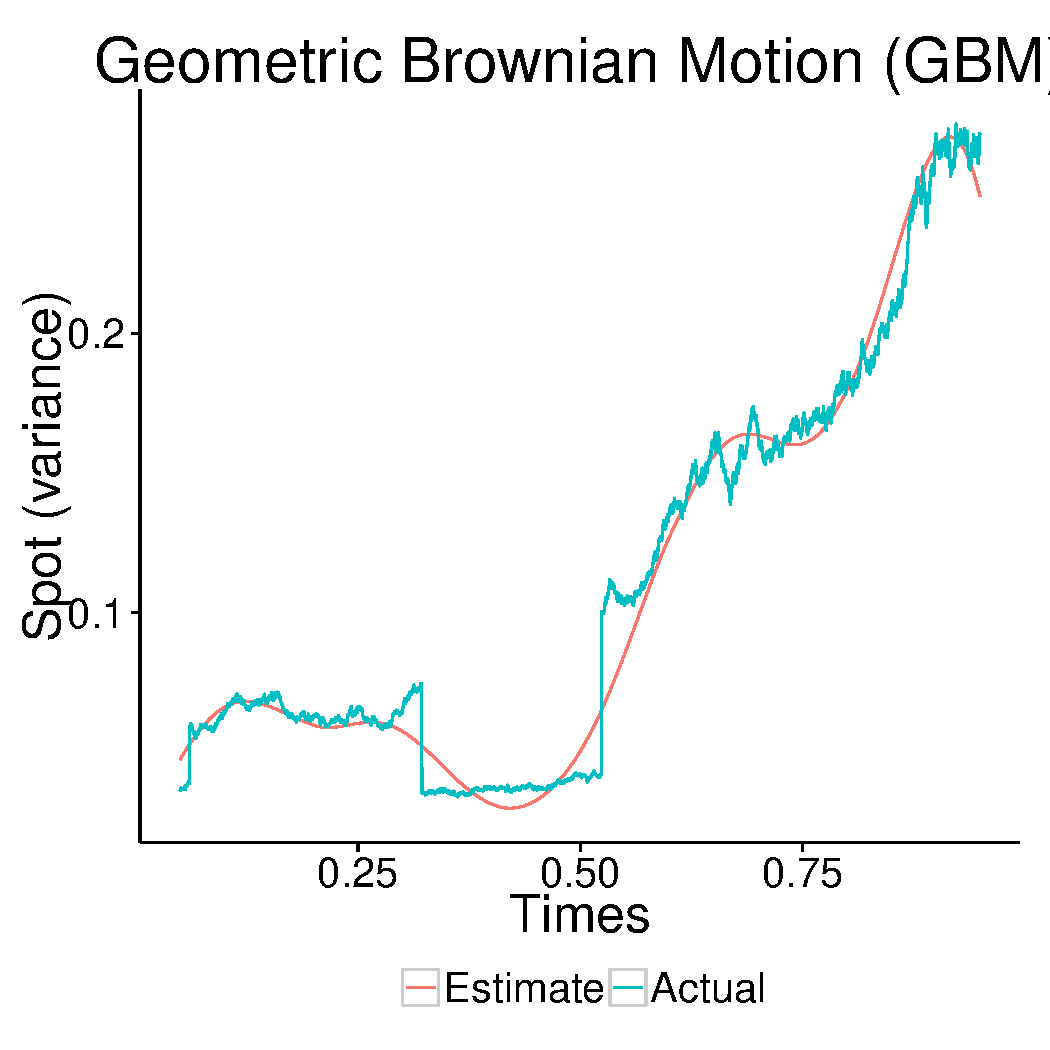
\includegraphics[width=0.45\textwidth]{/home/wale/Dropbox/Research/Paper3/pg.pdf}}}
  \qquad
  \subfloat[OU]{{ 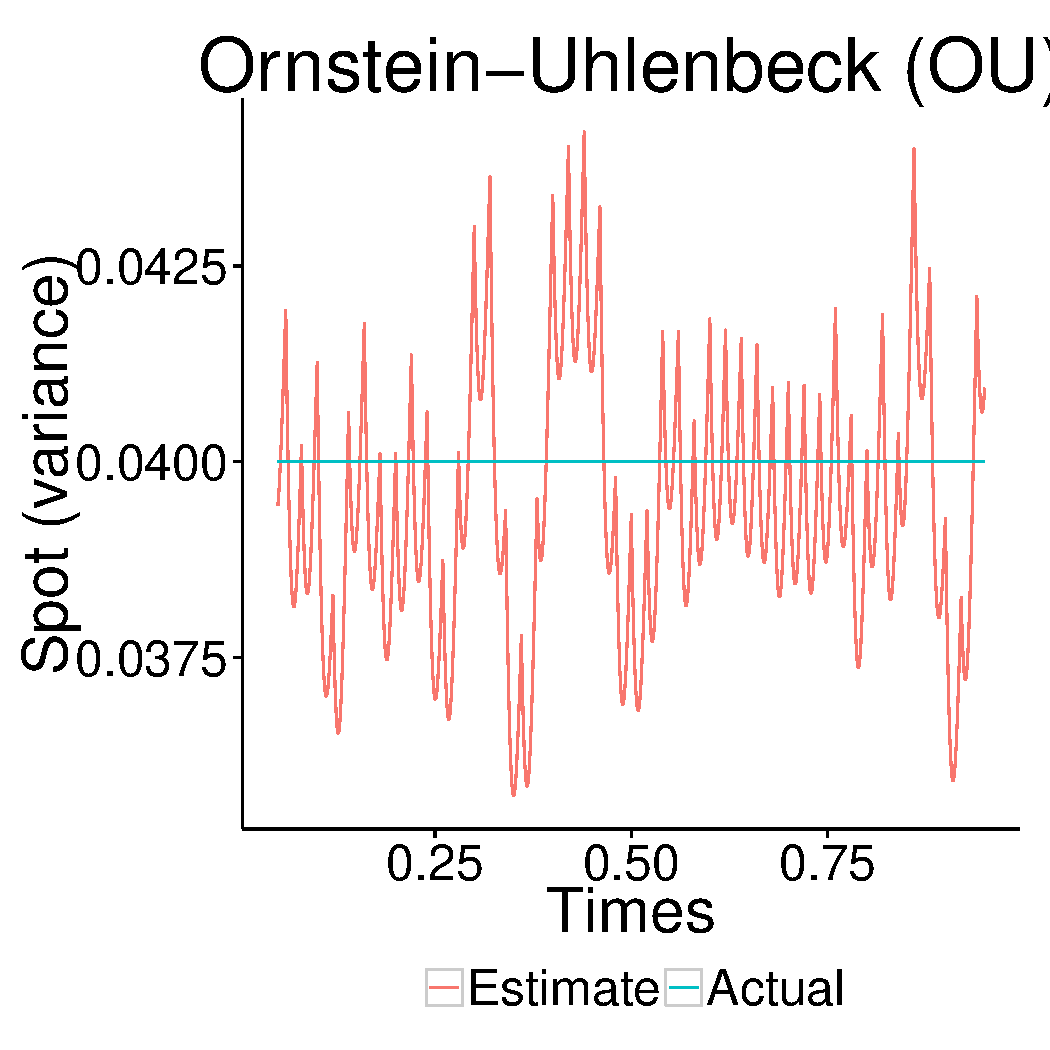
\includegraphics[width=0.45\textwidth]{/home/wale/Dropbox/Research/Paper3/po.pdf}}}
  \qquad
  \subfloat[ABM]{{ 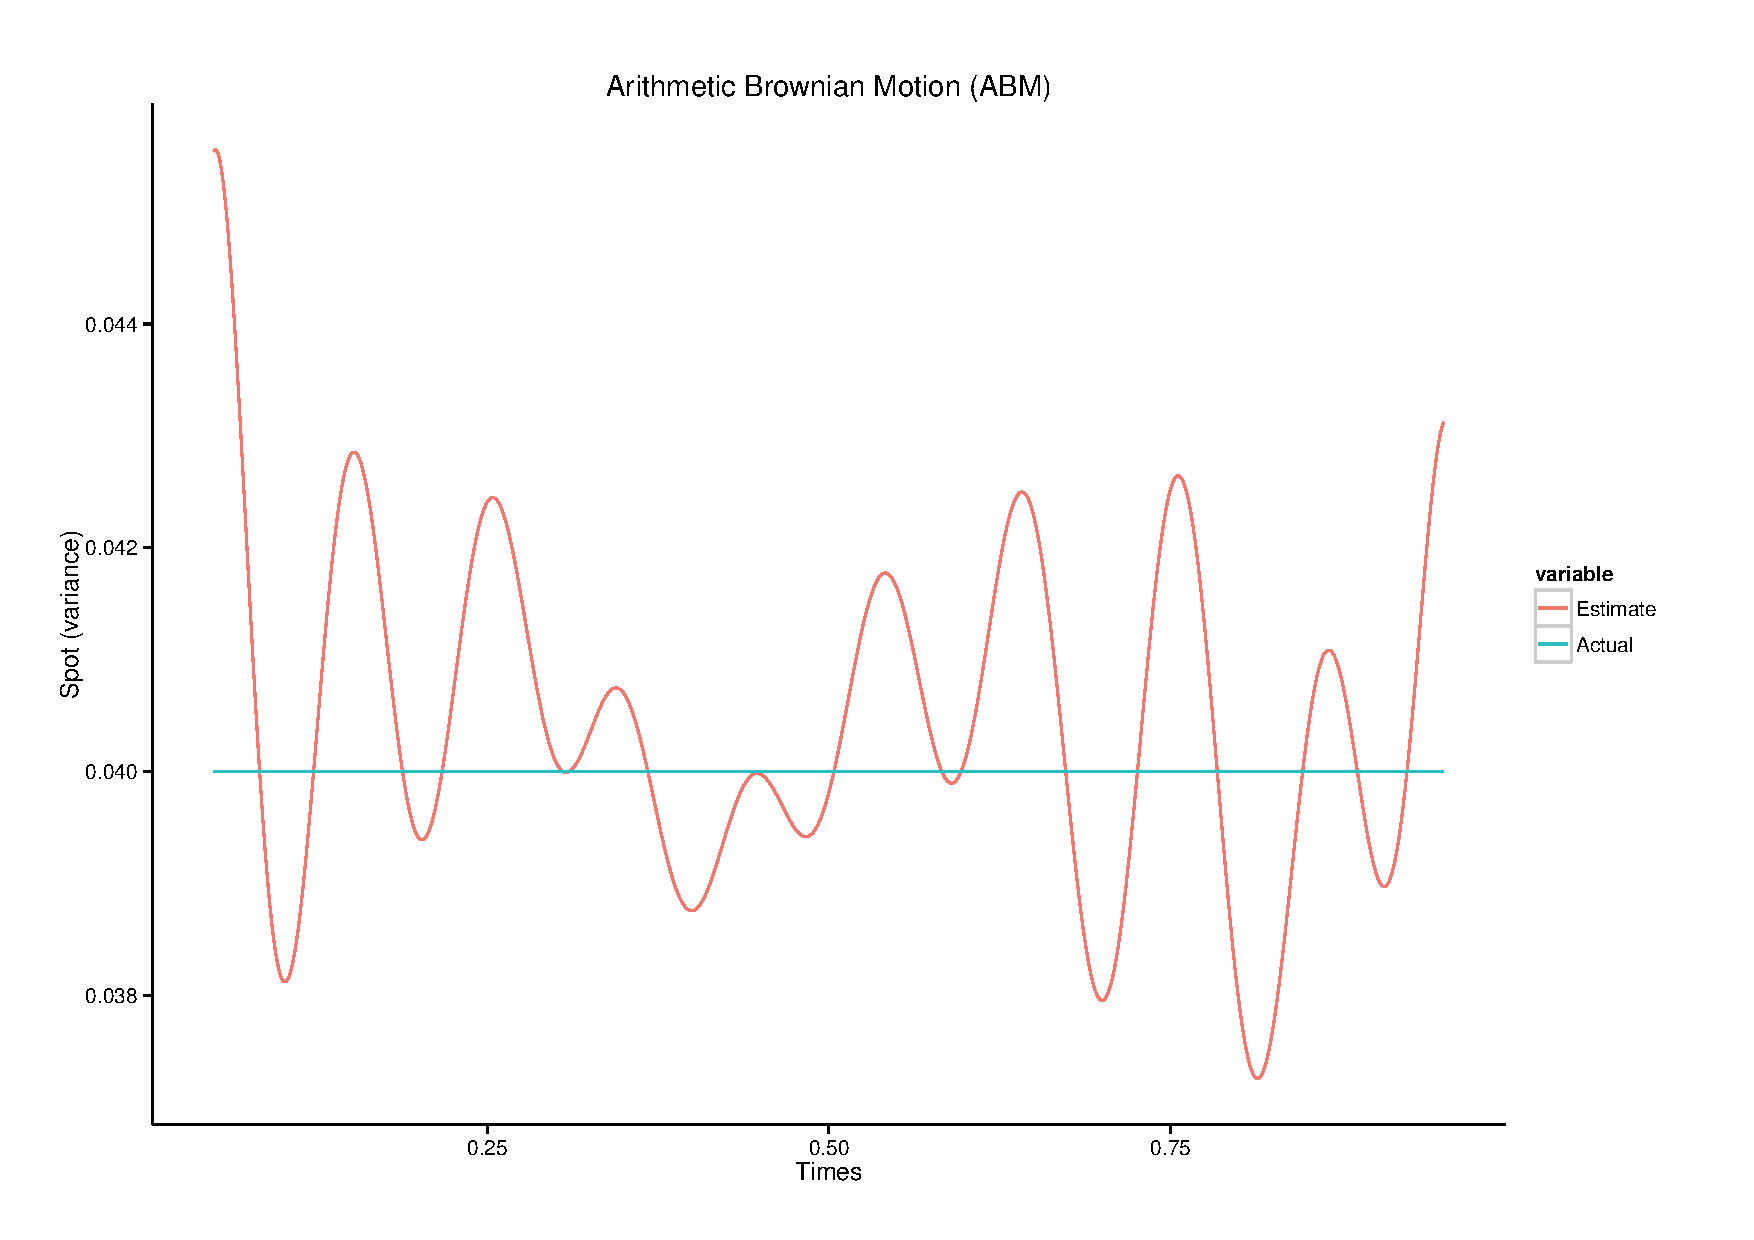
\includegraphics[width=0.45\textwidth]{/home/wale/Dropbox/Research/Paper3/pa.pdf}}}
  \subfloat[CIR]{{ 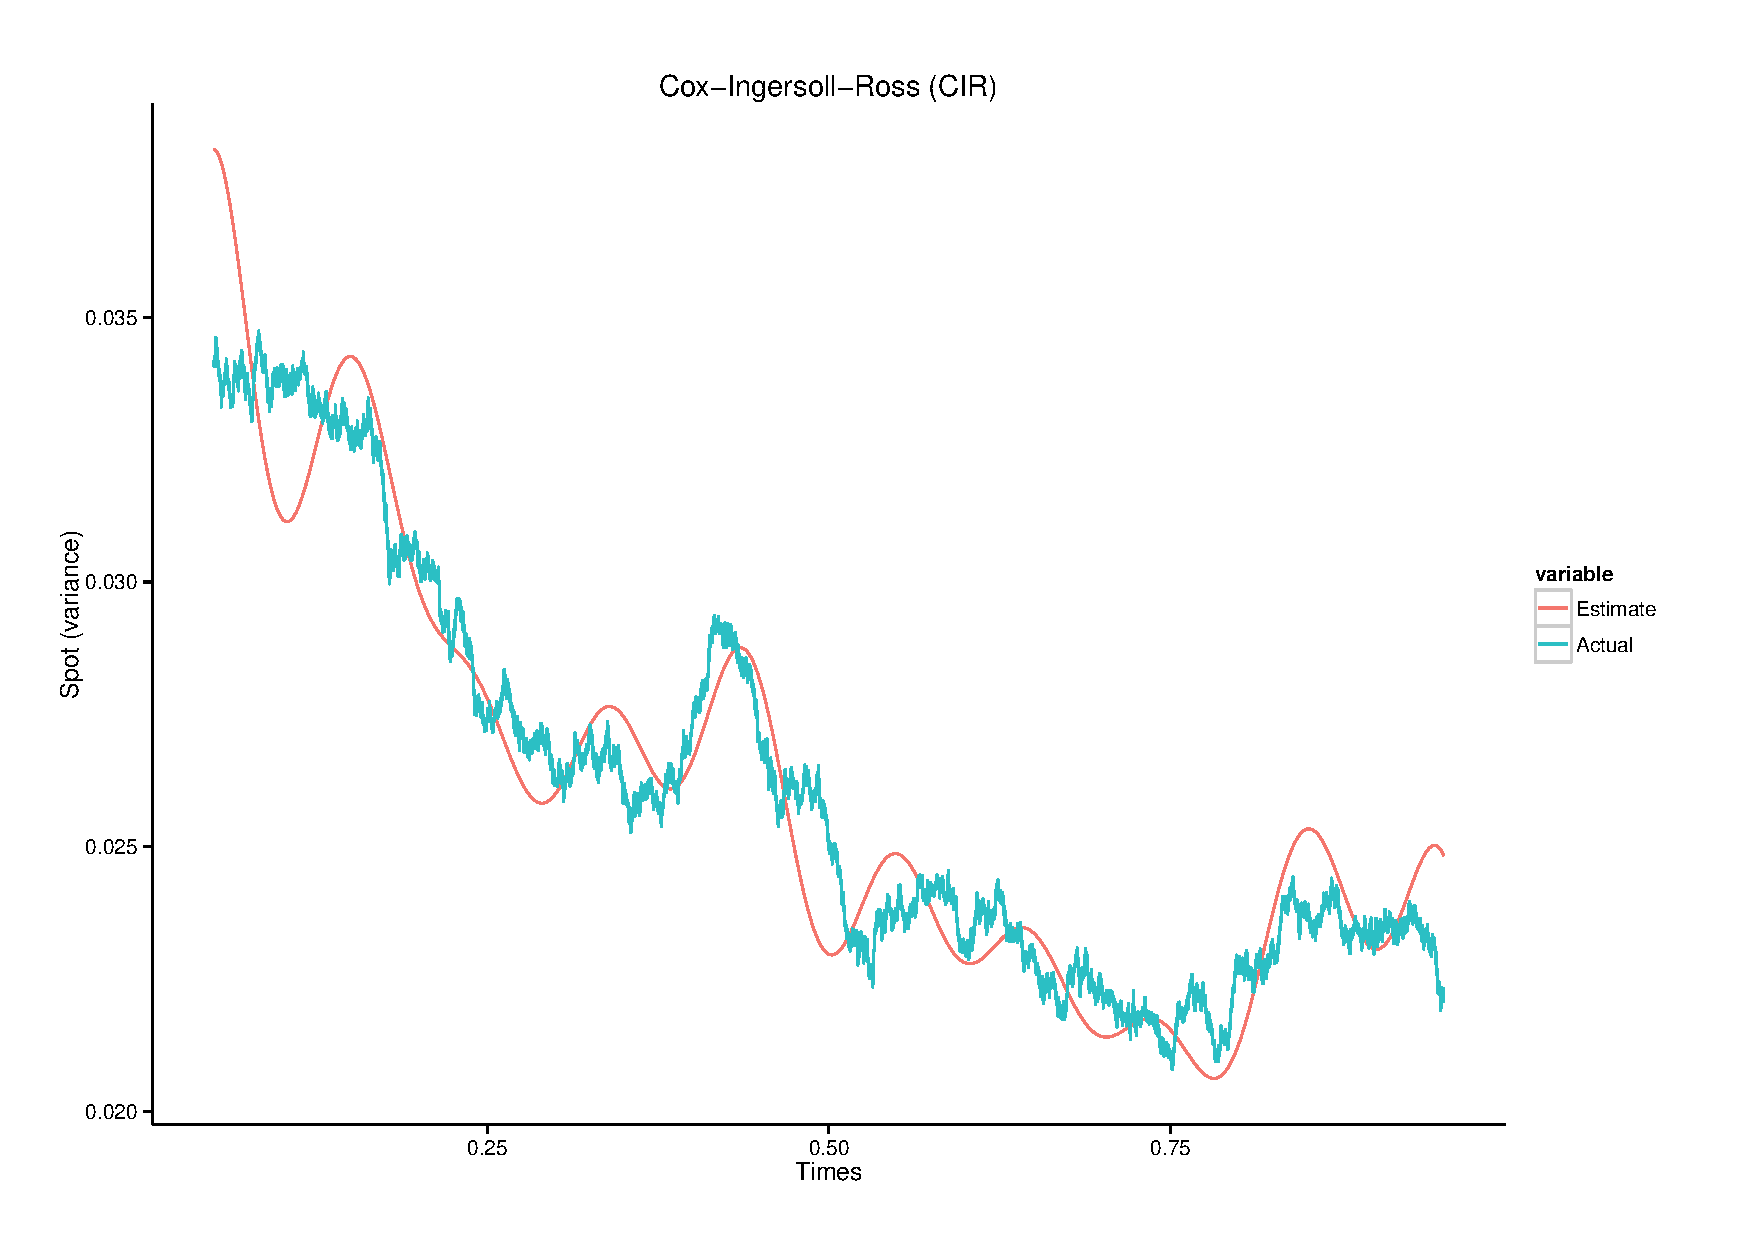
\includegraphics[width=0.45\textwidth]{/home/wale/Dropbox/Research/Paper3/pcir.pdf}}}
    \label{fig:path}
\end{figure}
}
    \framebreak
  \tiny{
    \begin{landscape}
\begin{table}[ht]
  %\tabcolsep=0.11cm
\begin{threeparttable}
  %\footnotesize
%\centering
  \caption{Mean integrated square error (MISE) of $\svnx$.\label{tab:mise}}
  
\begin{tabular*} {\columnwidth}{@{\extracolsep{\stretch{1}}}*{8}{r}@{}}
    \toprule 
   & \multicolumn{3}{c}{ABM} & &\multicolumn{3}{c}{OU}\\
    \cmidrule{2-4} 
    \cmidrule{5-8} 
\multicolumn{1}{c}{$n$} & \multicolumn{1}{c}{MISE} & \multicolumn{1}{c}{Sq. Bias} & \multicolumn{1}{c}{Var} && \multicolumn{1}{c}{MISE}& \multicolumn{1}{c}{Sq. Bias} & \multicolumn{1}{c}{Var}\\
    \midrule
500 & \num[scientific-notation=true,round-precision=3,round-mode=figures]{ 0.000129690514378747 } & \num[scientific-notation=true,round-precision=3,round-mode=figures]{ 2.86098860978027e-06 } & \num[scientific-notation=true,round-precision=3,round-mode=figures]{ 0.000126829525768967 } & & \num[scientific-notation=true,round-precision=3,round-mode=figures]{ 0.000142657171197515 } & \num[scientific-notation=true,round-precision=3,round-mode=figures]{ 1.19241391058862e-05 } & \num[scientific-notation=true,round-precision=3,round-mode=figures]{ 0.000130733032091629 } \\
5000 &\num[scientific-notation=true,round-precision=3,round-mode=figures]{ 1.41480010731752e-05 } & \num[scientific-notation=true,round-precision=3,round-mode=figures]{ 1.11112511718854e-06 } & \num[scientific-notation=true,round-precision=3,round-mode=figures]{ 1.30368759559867e-05 } & & \num[scientific-notation=true,round-precision=3,round-mode=figures]{ 1.44713297500796e-05 } & \num[scientific-notation=true,round-precision=3,round-mode=figures]{ 1.62292548526195e-06 } & \num[scientific-notation=true,round-precision=3,round-mode=figures]{ 1.28484042648177e-05 } \\ 
50000 &\num[scientific-notation=true,round-precision=3,round-mode=figures]{ 2.32308652636521e-06 } & \num[scientific-notation=true,round-precision=3,round-mode=figures]{ 1.02395100012948e-06 } & \num[scientific-notation=true,round-precision=3,round-mode=figures]{ 1.29913552623573e-06 } & & \num[scientific-notation=true,round-precision=3,round-mode=figures]{ 2.35629081189399e-06 } & \num[scientific-notation=true,round-precision=3,round-mode=figures]{ 1.12403547001524e-06 } & \num[scientific-notation=true,round-precision=3,round-mode=figures]{ 1.23225534187875e-06 } \\
   \midrule
  \end{tabular*}
\end{threeparttable}
\begin{threeparttable}
  %\footnotesize
%\centering
\begin{tabular*} {\columnwidth}{@{\extracolsep{\stretch{1}}}*{8}{r}@{}}
    \midrule
   & \multicolumn{3}{c}{GBM} & &\multicolumn{3}{c}{CIR}\\
    \cmidrule{2-4} 
    \cmidrule{5-8} 
\multicolumn{1}{c}{$n$} & \multicolumn{1}{c}{MISE} & \multicolumn{1}{c}{Sq. Bias} & \multicolumn{1}{c}{Var} && \multicolumn{1}{c}{MISE}& \multicolumn{1}{c}{Sq. Bias} & \multicolumn{1}{c}{Var}\\
    \midrule
500 & \num[scientific-notation=true,round-precision=3,round-mode=figures]{ 0.000217858539705785 } & \num[scientific-notation=true,round-precision=3,round-mode=figures]{ 4.17515036941201e-06 } & \num[scientific-notation=true,round-precision=3,round-mode=figures]{ 0.000213683389336373 } && \num[scientific-notation=true,round-precision=3,round-mode=figures]{ 6.25847666534302e-05 } & \num[scientific-notation=true,round-precision=3,round-mode=figures]{ 8.51220421884097e-07 } & \num[scientific-notation=true,round-precision=3,round-mode=figures]{ 6.17335462315461e-05 } \\ 

5000 & \num[scientific-notation=true,round-precision=3,round-mode=figures]{ 2.32787518909845e-05 } & \num[scientific-notation=true,round-precision=3,round-mode=figures]{ 1.58307630511742e-06 } & \num[scientific-notation=true,round-precision=3,round-mode=figures]{ 2.16956755858671e-05 } && \num[scientific-notation=true,round-precision=3,round-mode=figures]{ 6.82420050132428e-06 } & \num[scientific-notation=true,round-precision=3,round-mode=figures]{ 5.99985785058558e-07 } & \num[scientific-notation=true,round-precision=3,round-mode=figures]{ 6.22421471626572e-06 } \\
50000 & \num[scientific-notation=true,round-precision=3,round-mode=figures]{ 4.6593085666358e-06 } & \num[scientific-notation=true,round-precision=3,round-mode=figures]{ 1.01842335658939e-06 } & \num[scientific-notation=true,round-precision=3,round-mode=figures]{ 3.64088521004641e-06 } && \num[scientific-notation=true,round-precision=3,round-mode=figures]{ 1.45783049273178e-06 } & \num[scientific-notation=true,round-precision=3,round-mode=figures]{ 6.05894054142823e-07 } & \num[scientific-notation=true,round-precision=3,round-mode=figures]{ 8.51936438588961e-07 } \\
    \bottomrule
\end{tabular*}
  \medskip
  \footnotesize
Note: The mean of the integrated square errors are obtained by taking an average over 100 sample paths generated  for each  model/number of observations pair.
\end{threeparttable}
\end{table}

\end{landscape}
}
    \normalsize
  \framebreak
  \begin{theorem}
    $\hat{\sigma}^2_n$ converges in $L^2[0, T]$ in probability to $\sigma^2$ as $n \to \infty$.
      \end{theorem}
\end{frame}
%------------------------------------------------
\end{document} 
